\section{User-centered Design Research}

\subsection{Mockup-Studie: Bewertung der Benutzerfreundlichkeit und
Funktionalität}
Bei der Entwicklung eines nutzerzentrierten Designs steht die direkte Einbindung
der Zielgruppe im Mittelpunkt. Dieser Ansatz, der als User-Centered Design (UCD) 
bezeichnet wird, stellt die Integration der Bedürfnisse, Erwartungen und
Anforderungen der Benutzer in den Entwicklungsprozess in den Mittelpunkt. Ziel
ist es, Produkte und Anwendungen zu gestalten, die nicht nur funktional und
ästhetisch ansprechend sind, sondern auch die bestmögliche
Benutzerfreundlichkeit bieten.

\subsubsection{Methodik und Teilnehmende}
Im Rahmen des UCD-Prozesses wurde das zuvor in Kapitel \ref{sec:konzept}
vorgestellte Mockup-Konzept für den Studiengangsfinder entwickelt, das als
Prototyp diente. Um sicherzustellen, dass das entworfene Konzept den
Bedürfnissen der potenziellen Nutzer entspricht, wurde eine gezielte 
User-Centered-Design-Studie durchgeführt. Zu diesem Zweck wurden sechs
Studierende und Absolventen verschiedener Fachrichtungen eingeladen, den
Mockup-Entwurf zu evaluieren (siehe \autoref{table:teilnehmer-mockup-studie}).

\begin{table}[!ht]
    \centering
    \begin{tabular}{|l|l|l|l|}
        \hline
        \textbf{\#} & \textbf{Studienabschluss}                               & \textbf{Geschlecht} & \textbf{Datum} \\ \hline
        1           & Betriebswirtschaft B.A.                                 & Weiblich            & 16.09.2023     \\ \hline
        2           & Psychologie M.Sc.                                       & Weiblich            & 20.09.2023     \\ \hline
        3           & Informatik B.Sc.                                        & Männlich            & 25.09.2023     \\ \hline
        4           & Regenerative Energietechnik und Energieeffizienz B.Eng. & Männlich            & 07.10.2023     \\ \hline
        5           & Bioprozessinformatik B.Sc.                              & Männlich            & 08.10.2023     \\ \hline
        6           & Betriebswirtschaft B.A.                                 & Weiblich            & 12.10.2023     \\ \hline
    \end{tabular}

    \caption{Probanden der Mockup-Studie}
    \label{table:teilnehmer-mockup-studie}
\end{table}

\subsubsection{Ablauf des Tests}
Die Studie wurde in Form von Einzelinterviews durchgeführt. Die Teilnehmer wurden ermutigt, ihre persönlichen Perspektiven, Erfahrungen und Vorschläge einzubringen. Außerdem wurden sie gebeten, ihre Gedanken zum Entwurf laut zu äußern. Anschließend wurden ihnen nacheinander alle Grafiken des Entwurfs gezeigt (1. \autoref{fig:mockup-bubbles},
2. \autoref{fig:mockup-bubbles-hover}, 3. \autoref{fig:mockup-bubbles-popup}). 

Offene Fragen zu Designelementen, Verständlichkeit von Informationen und allgemeinen Nutzererfahrungen sollten Aufschluss über mögliche Stärken und Schwächen des Design-Proto\-typs geben. Ziel war es, frühzeitig wertvolles Feedback zu erhalten, um Optimierungen und Anpassungen vornehmen zu können, bevor die Umsetzung in die nächste Phase geht. Die lauten Gedanken der Teilnehmerinnen und Teilnehmer wurden von Herrn Huber in einem Freitextfeld dokumentiert.

\subsubsection{Ergebnisse der Mockup-Studie}
Die Rückmeldungen der Studienteilnehmenden lassen sich in folgende konsistente
Muster zusammenfassen.

\paragraph{Bild 1: Visualisierung der Studiengänge}
Die Übersichtskarte wurde von den Teilnehmenden als unübersichtlich und geclustert wahrgenommen. Besonders die Farbähnlichkeit der Studiengänge wurde als störend
empfunden.

Eine konkrete Verbesserungsmöglichkeit besteht darin, die Überschriften der Nebel zu vergrößern und fett darzustellen, um die Lesbarkeit zu verbessern. Darüber hinaus wurde vorgeschlagen, alle Abkürzungen der Studiengänge standardmäßig auszublenden und nur den Nebel zu beschriften, um die Übersichtlichkeit zu erhöhen. Sobald der Benutzer mit der Maus in die Nähe des Nebels kommt, sollte die Überschrift des Nebels ausgeblendet und die Abkürzungen aller darin enthaltenen Studiengänge eingeblendet werden. Um die Zufälligkeit und Ähnlichkeit der Farben zu vermeiden, könnten die Studiengänge in den Fakultätsfarben und der Nebel im Hintergrund neutral (z.B. grau) eingefärbt werden.

\paragraph{Bild 2: Interaktivität}
Das Hover-Event über eine Bubble mit einem Tooltip wurde durchweg als passend und verständlich betrachtet. Dieses Element wurde von den Teilnehmenden als intuitiv und funktional empfunden.

\paragraph{Bild 3: Popup mit Details eines Studiengangs}
Über die Anordnung der Informationen im Popup gingen die Meinungen auseinander. Während einige eine absteigende Sortierung nach Relevanz bevorzugten, sprachen sich andere für eine alphabetische Sortierung aus. Positiv bewertet wurde die Funktion, ähnliche Studiengänge nach Ähnlichkeit zu sortieren. Die Darstellung der Branchen wurde als weniger aussagekräftig empfunden und teilweise vorgeschlagen, diese Information zu entfernen. Die Möglichkeit, sich Unternehmen in Regensburg anzeigen zu lassen, wurde positiv bewertet und es wurde angeregt, diese Funktion ausklappbar zu gestalten, um die Übersichtlichkeit zu erhöhen. Es wurde außerdem empfohlen, die Informationen zu den Einstiegsgehältern zu erläutern, möglicherweise durch die Integration von Fragezeichensymbolen und Tooltips.

\paragraph{Generelle Anmerkungen}
Zu den allgemeinen Verbesserungsvorschlägen gehören ein besserer Farbkontrast, mehr Erläuterungen zu verschiedenen Informationen und eine einheitliche und intuitive Anordnung der Designelemente, um die Übersichtlichkeit insgesamt zu erhöhen.

%
%
%
%
%
%
% PROTOTYPEN STUDIE
\subsection{Prototypen-Studie: Evaluation durch Studieninteressierte}
Nach der Entwicklung des Prototyps auf Basis des Mockups und der Erkenntnisse aus der Mockup-Studie wurden Studieninteressierte eingeladen, den Prototyp von StudyMap zu testen. Nach der selbstständigen Interaktion mit dem Prototyp wurden die Teilnehmenden gebeten, an einer Umfrage teilzunehmen, um ihre Erfahrungen, Meinungen und Verbesserungsvorschläge zu dokumentieren.

Der folgende Abschnitt beleuchtet die Methodik, den genauen Ablauf des Tests und stellt die Ergebnisse dieser Evaluationsstudie vor, die wertvolle Einblicke in die Effektivität und Benutzerfreundlichkeit des Prototyps liefert.

\subsubsection{Methodik und Teilnehmende}
Der nächste Schritt im UCD-Prozess ist das Testen des Prototyps mit potenziellen Nutzern, d.h. Studieninteressierten. Zu diesem Zweck wurde auf der Grundlage des Mockups und der im vorherigen Kapitel beschriebenen Mockup-Studie ein Prototyp entwickelt. Ziel dieser Studie ist es, frühe Designentscheidungen zu hinterfragen und das Tool auf Usability zu testen. Der Vorteil einer solch frühen Evaluierung ist, dass größere Änderungen am Endprodukt wesentlich aufwendiger sind als in einem frühen Entwicklungsstadium.

An der Studie nahmen 40 Schülerinnen und Schüler der 11. Klasse des Johannes-Nepomuk-Gymnasiums in Rohr i.NB teil. Alle diese Schüler werden voraussichtlich im Jahr 2026 die allgemeine Hochschulreife erlangen und entsprechen damit genau der Zielgruppe eines Studiengangfinders. Durch die örtliche Nähe des Gymnasiums zur OTH-Regensburg ist die Eignung des Teilnehmerkreises zusätzlich gegeben.

Die Befragung fand in zwei Gruppen (Klasse 11A und Klasse 11B) im Johannes-Neopomuk-Gymnasium vor Ort im Computerraum der Schule statt. Dort konnten die Schülerinnen und Schüler an den Windows-Rechnern der Schule sowohl den Prototyp testen als auch die Umfrage in Einzelarbeit beantworten.

\subsubsection{Ablauf des Tests}
Die Studie begann mit einer kurzen Einführung, in der den Teilnehmenden der
Zweck der Studie und die Handhabung des Prototyps erläutert wurden. Anschließend
wurden die Teilnehmenden gebeten, den Prototyp selbst zu verwenden und zwei
Aufgaben innerhalb einer Online-Umfrage zu lösen, um die Benutzerfreundlichkeit, die Navigationsstruktur und
die Funktionalitäten des Studiengangsfinders zu testen (siehe
\autoref{fig:prototyp-umfrage-aufgaben}). In dieser Phase wurden sowohl
quantitative als auch qualitative Daten erhoben, um ein umfassendes Bild der 
Benutzererfahrung zu erhalten.

\begin{figure}[H]
    \centering
    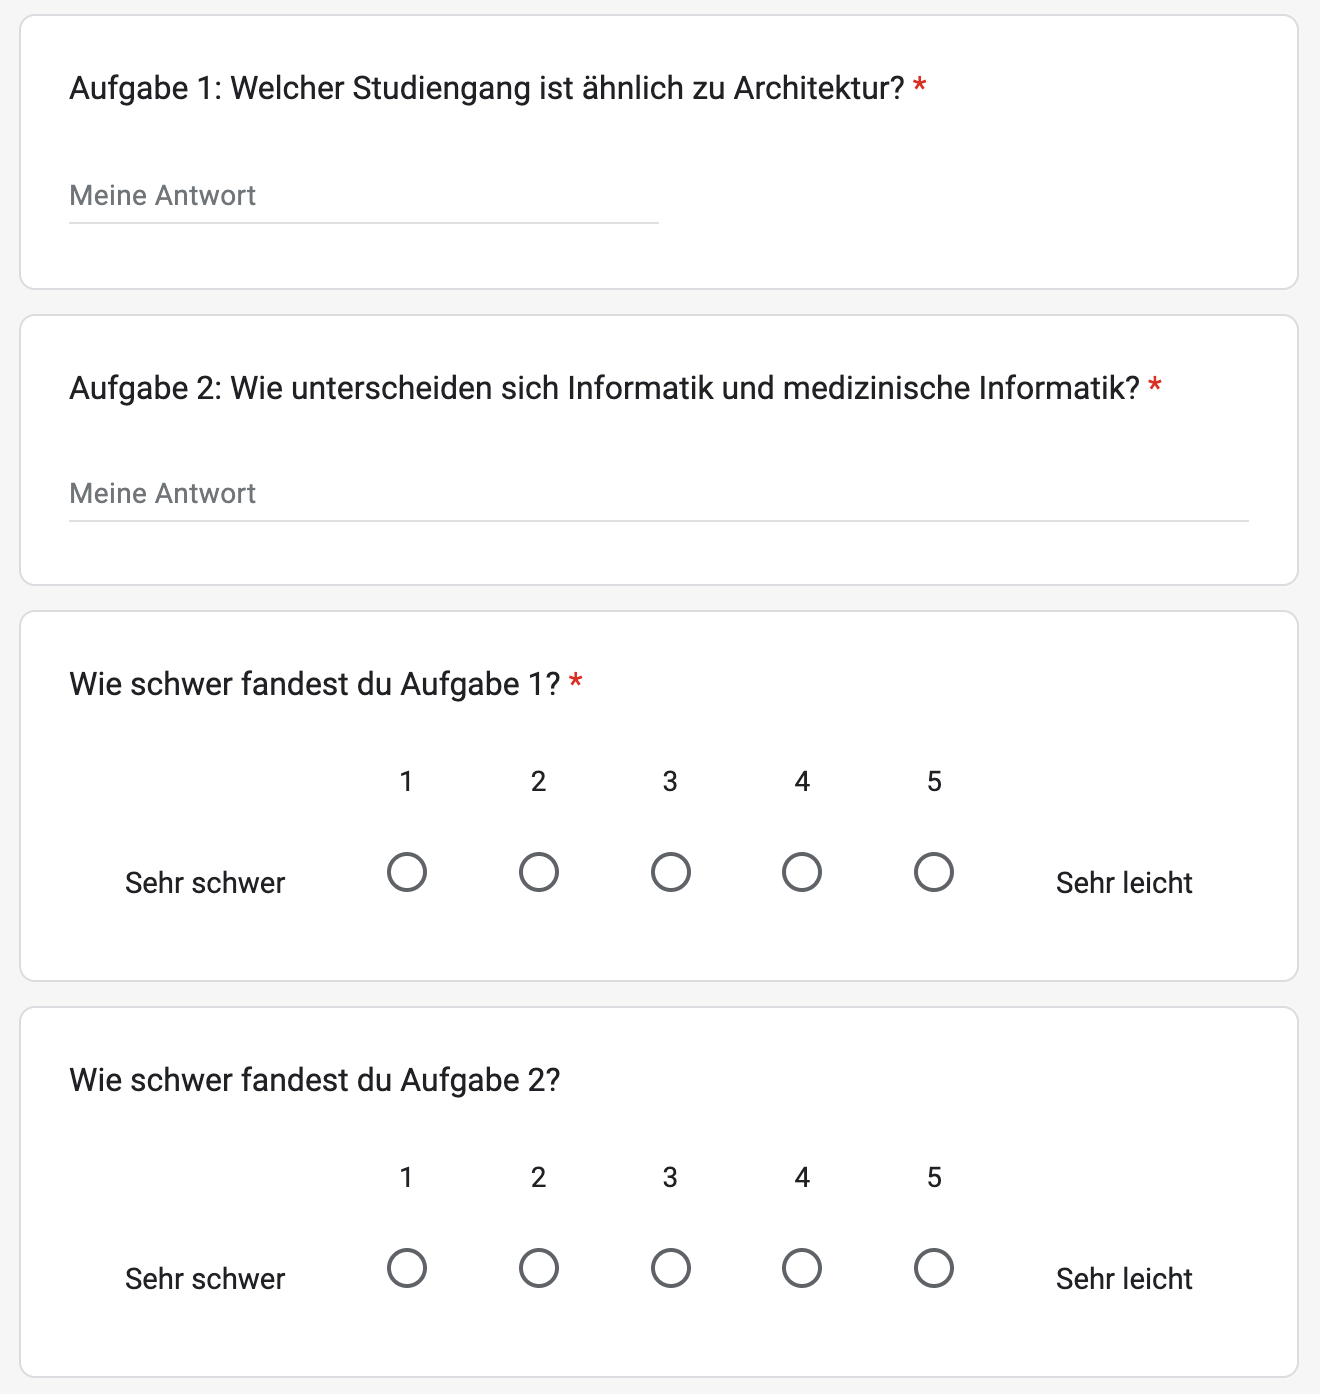
\includegraphics[width=0.5\textwidth]{umfrage_aufgaben}
    \caption{Prototypen-Studie: Aufgaben}
    \bildquelle{Eigene Darstellung}
    \label{fig:prototyp-umfrage-aufgaben}
\end{figure}

Nach der Interaktion mit dem Prototyp wurden die Teilnehmenden gebeten, zusätzlich zu den Aufgaben weitere Fragen in der anonymen Online-Umfrage zu beantworten.

Die ersten Fragen der Umfrage waren Multiple-Choice-Fragen mit den Antwortmöglichkeiten \glqq Ja\grqq{}, \glqq Nein\grqq{} und \glqq Keine Angabe\grqq{}.

\begin{enumerate}
    \item Willst du nach dem Abi studieren?
    \item Wenn ja, weißt du schon, was für ein Studium?
    \item Würde dir StudyMap bei der Wahl des Studiengangs helfen?
    \item Die Antwort hier ist "Ja" (Aufmerksamkeitsfrage)
\end{enumerate}

Danach folgten die beiden oben beschriebenen Aufgaben (siehe
\autoref{fig:prototyp-umfrage-aufgaben}). Zuletzt wurden die folgenden Fragen
mit Freitextfeldern zur Beantwortung gestellt:

\begin{enumerate}
    \item Was findest du an dem Konzept gut?
    \item Was findest du am Konzept schlecht?
    \item Hast du neue Ideen für den Prototyp?
    \item Wenn du bei \glqq Würde StudyMap dir bei der Studienwahl helfen?\grqq{} NEIN angekreuzt hast: Warum nicht?
\end{enumerate}

Die Fragen wurden bewusst mit Freitextfeldern zur Beantwortung versehen, um den Teilnehmenden die Möglichkeit zu geben, mit allen möglichen Gedankengängen zu antworten. Dies kann dazu führen, dass Ideen entstehen, die bisher noch nicht bedacht wurden und somit im Endprodukt umgesetzt werden können. Die Befragung dauerte ca. 15 Minuten. Durch die Kombination der Interaktion mit dem Prototyp und der schriftlichen Befragung konnten vielfältige Einblicke in die Nutzerperspektive gewonnen werden.

\subsubsection{Ergebnisse der Prototypen-Studie}

\subsection{Zusammenfassung der Studien}